%%=============================================================================
%% Methodologie
%%=============================================================================

\chapter{\IfLanguageName{dutch}{Methodologie}{Methodology}}%
\label{ch:methodologie}

%% TODO: In dit hoofstuk geef je een korte toelichting over hoe je te werk bent
%% gegaan. Verdeel je onderzoek in grote fasen, en licht in elke fase toe wat
%% de doelstelling was, welke deliverables daar uit gekomen zijn, en welke
%% onderzoeksmethoden je daarbij toegepast hebt. Verantwoord waarom je
%% op deze manier te werk gegaan bent.
%% 
%% Voorbeelden van zulke fasen zijn: literatuurstudie, opstellen van een
%% requirements-analyse, opstellen long-list (bij vergelijkende studie),
%% selectie van geschikte tools (bij vergelijkende studie, "short-list"),
%% opzetten testopstelling/PoC, uitvoeren testen en verzamelen
%% van resultaten, analyse van resultaten, ...
%%
%% !!!!! LET OP !!!!!
%%
%% Het is uitdrukkelijk NIET de bedoeling dat je het grootste deel van de corpus
%% van je bachelorproef in dit hoofstuk verwerkt! Dit hoofdstuk is eerder een
%% kort overzicht van je plan van aanpak.
%%
%% Maak voor elke fase (behalve het literatuuronderzoek) een NIEUW HOOFDSTUK aan
%% en geef het een gepaste titel.
In de initiële fase van mijn onderzoek, de literatuurstudie, heb ik me gericht op het verzamelen van de bestaande 
kennis en onderzoek op het gebied van webapplicatiebeveiliging, 
pentesting-tools en frameworks, met een specifieke focus op WordPress en Laravel. Deze fase was van cruciaal 
belang om een stevige basis te leggen voor mijn onderzoek en om de context en achtergrond van het onderwerp volledig te 
begrijpen.

Om dit te bereiken, heb ik verschillende bronnen geraadpleegd, waaronder wetenschappelijke artikelen, boeken  
en rapporten van bekende instellingen en experts op het gebied van cybersecurity. 
Ik heb zoekopdrachten uitgevoerd in diverse academische databases, zoals PubMed, research gate en 
Google Scholar, om relevante literatuur te op nemen in mijn studie. Deze literatuur heb ik grondig geanalyseerd en 
samengevat, waarbij ik de nadruk legde op recente ontwikkelingen, trends en mogelijke tekortkomingen in de bestaande kennis.
Ook heeft de literatuur het globale aspect van cybersecutiy onder de loep genomen waardoor er een zeer duidelijk begrip is gekomen 
van wat er moet gebeuren en waarom.

\section{\IfLanguageName{dutch}{Requirements Analyse}{Requirements analysis}}
De requirements analyse beschrijft de methoden en technieken die worden toegepast voor het uitvoeren van penetratietests op drie 
verschillende webomgevingen: een WordPress-applicatie zonder beveiligingsplugins, een WordPress-applicatie met 
beveiligingsplugins, en een Laravel-applicatie. Het doel van deze tests is om kwetsbaarheden te identificeren, te 
analyseren en de effectiviteit van de beveiligingsmaatregelen in de verschillende omgevingen te vergelijken.
Deze 3 webomgevingen worden geselecteerd op basis van hun populariteit en relevantie voor kleine tot middelgrote bedrijven 
zoals Sinergio wiens ook mijn doelgroep is.

Voorafgaand aan de uitvoering van de penetratietests wordt toestemming verkregen van de beheerders van de 
webomgevingen. Er wordt een veilige testomgeving opgezet om de impact op de live systemen te minimaliseren. 
Alle tests worden uitgevoerd in overeenstemming met de ethische richtlijnen voor cybersecurity onderzoek, 
waarbij de integriteit van de geteste systemen voorop staat.

Voor dit onderzoek worden drie verschillende penetratietesttools ingezet, elk geselecteerd vanwege hun 
specifieke sterktes in het identificeren en exploiteren van bepaalde soorten kwetsbaarheden:

\begin{itemize}
    \item Tool 1 wordt gebruikt voor de eerste webomgeving, een WordPress-applicatie zonder 
    beveiligingsplugins. Deze tool moet bijzonder geschikt voor het detecteren van webgebaseerde kwetsbaarheden 
    zoals SQL-injecties en cross-site scripting (XSS), waardoor het een uitstekende keuze is voor 
    een basis WordPress-installatie.
    \item Tool 2 wordt ingezet voor de tweede webomgeving, een WordPress-applicatie met beveiligingsplugins. 
    Deze tool excelleert in het omzeilen van beveiligingsmaatregelen en het uitvoeren van geautomatiseerde 
    aanvallen, waaronder brute force aanvallen. Dit maakt het bijzonder geschikt voor het grondig 
    testen van beveiligde WordPress-installaties.
    \item Tool 3 wordt gekozen voor de derde webomgeving, een Laravel-applicatie. Deze tool staat 
    bekend om zijn vermogen om specifieke framework-kwetsbaarheden te exploiteren en biedt functionaliteiten 
    die cruciaal zijn voor het testen van complexe applicaties zoals die gebouwd met Laravel.
\end{itemize}

Alle resultaten van de tests worden verzameld en gedocumenteerd. De data wordt geanalyseerd 
om de ernst en de impact van elke gevonden kwetsbaarheid te bepalen. Deze analyse helpt niet alleen bij 
het identificeren van de zwakke punten binnen elke webomgeving, maar ook bij het vergelijken van de 
veiligheid tussen de verschillende systemen. Ook word er gekeken naar de gebruiksvriendelijkheide en 
effectiviteit van de testen door een brute force aanval te simuleren op de wordpress applicatie met beveiligingsplugins.

\section{\IfLanguageName{dutch}{Keuze van Penetratietesttools}{Selection of pentesttools}}
In het kader van dit onderzoek naar de beveiliging van drie verschillende webomgevingen is de keuze van 
de juiste penetratietesttools cruciaal. Voor elk van deze omgevingen is een tool geselecteerd die het 
best past bij de specifieke kenmerken en beveiligingsuitdagingen. De geselecteerde tools zijn 
Metasploit, Burp Suite en OWASP ZAP. Hieronder volgt een verklaring van waarom deze tools 
bijzonder geschikt zijn voor dit onderzoek.
\begin{figure}
    \centering
    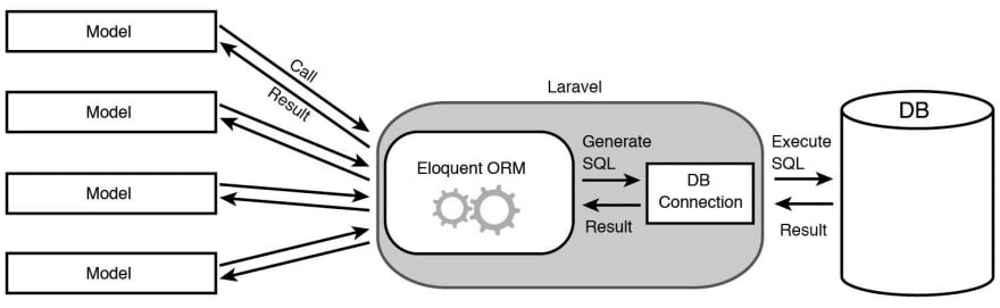
\includegraphics[height=0.2\textheight]{laravel_schema.png}
    \caption[Laravel ORM schema (Eloquent)]{Laravel ORM shema (Eloquent)}
\end{figure}
\subsection{\IfLanguageName{dutch}{Metasploit voor de Laravel-applicatie}{Metasploit for the Laravel application}}
Metasploit is een van de meest uitgebreide frameworks voor het uitvoeren van penetratietests en 
staat bekend om zijn robuuste exploit-database en modulaire aanpak. De Laravel-applicatie, bekend 
om zijn rijke set aan functionaliteiten en complexe architectuur, kan profiteren van Metasploit's 
vermogen om specifieke exploits te gebruiken die zijn afgestemd op gedetecteerde kwetsbaarheden. 
De tool biedt geautomatiseerde exploitatie technieken die essentieel zijn voor het identificeren 
van beveiligingsrisico's in een geavanceerd framework zoals Laravel. Bovendien ondersteunt 
Metasploit de ontwikkeling van aangepaste exploits, wat van grote waarde kan zijn bij 
het testen van maatwerkfuncties binnen de Laravel-applicatie.

\subsection{\IfLanguageName{dutch}{Burp Suite voor de wordpress applicatie met beveiligings plugins}{Burp Suite for the wordpress application with security plugins}}
Burp Suite, een geïntegreerd platform voor het testen van de beveiliging van webapplicaties, is 
bijzonder effectief voor het analyseren van HTTP-verkeer en het uitvoeren van geavanceerde web 
aanvallen. Voor een WordPress-installatie met beveiligingsplugins biedt Burp Suite de noodzakelijke 
diepgang om de effectiviteit van deze plugins te evalueren. Door zijn vermogen om verzoeken te 
onderscheppen, te manipuleren en opnieuw te versturen, kunnen testers de robuustheid van 
beveiligingsmaatregelen zoals firewalls en inbraakdetectiesystemen die door plugins worden 
geïmplementeerd, nauwkeurig beoordelen. Burp Suite's scanner (bij de enterprise edition) kan automatisch een breed scala 
aan kwetsbaarheden identificeren, wat tijd bespaart tijdens de testfase en zorgt voor een 
grondige evaluatie van de beveiligingsstatus.

\subsection{\IfLanguageName{dutch}{OWASP ZAP voor de wordpress applicatie zonder beveiligings plugins}{OWASP ZAP for the wordpress application without security plugins}}
OWASP ZAP (Zed Attack Proxy) is een open-source tool voor het automatisch vinden van beveiligingsfouten 
in webapplicaties tijdens het ontwikkelings- en testproces. Gezien zijn reputatie en uitgebreide 
ondersteuning door de OWASP-community is ZAP bijzonder geschikt voor het testen van een 
WordPress-site zonder aanvullende beveiligingsmaatregelen. ZAP's geïntegreerde scanner en 
intercepting proxy maken het eenvoudig om kwetsbaarheden zoals XSS en SQL-injectie aan te 
tonen, die voorkomen in basisconfiguraties van WordPress. Daarnaast biedt ZAP dynamische 
analyse van de applicatie in real-time, wat helpt bij het direct identificeren van beveiligingsproblemen.


\section{\IfLanguageName{dutch}{Proof of Concept: Gebruiksvriendelijkheid en Effectiviteit van Pentesting Tools voor Webapplicaties}{Proof of Concept: Usability and Effectiveness of Pentesting Tools for Web Applications}}

In de proof of concept testen we drie verschillende webomgevingen met pentesting tools om hun bruikbaarheid en effectiviteit te evalueren. 
Deze benadering is gericht op het vergelijken van de uitkomsten van pentests in elke omgeving, waardoor we kunnen vaststellen hoe de 
beveiligingsuitdagingen en kwetsbaarheden verschillen.

\subsubsection{\IfLanguageName{dutch}{Omgevingsdiversiteit}{Environmental diversity}}
De aanpak in deze proof of concept is gebaseerd op een holistische benadering, waarbij een scala aan pentesting tools wordt gebruikt die zijn afgestemd 
op de unieke kenmerken van elke omgeving. Het team van Sinergio begrijpt dat geen twee webomgevingen hetzelfde zijn, en daarom is het essentieel om een breed scala 
aan tools in te zetten om alle mogelijke kwetsbaarheden en beveiligingsrisico's aan het licht te brengen.

Door deze diversiteit aan tools kan het team niet alleen de specifieke omgeving testen met de best passende tool, maar ook de algehele robuustheid en 
weerbaarheid van de systemen maximaliseren. Elke tool heeft zijn eigen sterke punten en specialiteiten, waardoor een uitgebreide evaluatie mogelijk 
is die verder gaat dan alleen de oppervlakte.

Door te variëren in de gebruikte tools, kan het team verschillende aanvalsscenario's simuleren en de reactie van de systemen daarop beoordelen. Dit 
stelt hen in staat om een diepgaand inzicht te krijgen in de beveiligingsstatus van elke omgeving en biedt waardevolle informatie voor het verbeteren 
van de algehele beveiliging.

\subsubsection{\IfLanguageName{dutch}{Focus van pentesttools}{Focus of the pentesttools}}
De evaluatie van de beveiligingsplugin omvat het gebruik van Burp Suite om de efficiëntie te testen. De focus ligt op het evalueren van de weerstand 
tegen veelvoorkomende webaanvallen, zoals brute force-aanvallen en SQL-injectie. Ze analyseren hoe de plugin potentiële dreigingen behandelt met 
behulp van Burp Suite en identificeren eventuele tekortkomingen in de bescherming

OWASP ZAP helpt bij het blootleggen van kwetsbaarheden die een website zonder beveiligingsmaatregelen zou kunnen hebben. De nadruk ligt op het 
ontdekken van eenvoudig te exploiteren kwetsbaarheden en het bieden van educatie aan nieuwe gebruikers om deze kwetsbaarheden te begrijpen en 
te leren hoe ze te mitigeren.

Met Metasploit wordt gefocust op geavanceerdere beveiligingsaspecten, zoals routebescherming en authenticatiemechanismen.
In Laravel is het ook mogelijk om het aantal inlogpogingen instellen voordat een gebruiker tijdelijk wordt geblokkeerd. Dit wordt vaak gedaan 
als een beveiligingsmaatregel om brute force-aanvallen te voorkomen. Je kunt het aantal inlogpogingen aanpassen door een eigenschap genaamd 
'maxAttempts' in te stellen in de configuratie van het authenticatiesysteem van Laravel. Deze tests zullen 
bijdragen aan het inzicht in de robuustheid van de beveiliging en helpen bij het identificeren van potentieel over het hoofd geziene kwetsbaarheden.
